% Typeset with XeTeX
% Allows use of system fonts rather than just LaTeX's ones
% NOTE - if you use TeXShop and Bibdesk (Mac), can complete citations
%  - open your .bib file, type~\citep{xx... and then F5 or Option-Escape
\documentclass[11.5pt]{article}
\usepackage[width=6.5in,height=10in]{geometry} % set page layout
\geometry{a4paper}  % or a4paper
\usepackage[xetex]{graphicx} % allows us to manipulate graphics.
% Replace option [] with pdftex if you don't use Xe(La)TeX
\usepackage{color}
\usepackage{indentfirst}
\usepackage{epstopdf} % automatic conversion of eps to pdf 
\usepackage{amsmath, amssymb} % Better maths support & more symbols
\usepackage{textcomp} % provide lots of new symbols - see textcomp.pdf
% line spacing: \doublespacing, \onehalfspacing, \singlespacing
\usepackage{setspace}
\singlespacing
\usepackage{pgfplotstable}
% allows text flowing around figs
% use \begin{wrapfigure}{x}{width} where x = r(ight) or l(eft)
\usepackage{wrapfig}
\usepackage[parfill]{parskip} % don't indent new paragraphs
\usepackage{flafter}  % Don't place figs & tables before their definition 
\usepackage{verbatim} % allows \begin and \end{comment} regions
\usepackage{booktabs} % makes tables look good
\usepackage{bm}  % Define \bm{} to use bold math fonts
% linenumbers in L margin, start & end with \linenumbers \nolinenumbers,
\usepackage{lineno} % use option [modulo] for steps of 5
\usepackage[auth-sc]{authblk} % authors & institutions - see authblk.pdf
\renewcommand\Authands{ and } % separates the last 2 authors in the list
% control how captions look; here, use small font and indent both margins by 20pt
\usepackage[small]{caption} 
\setlength{\captionmargin}{20pt}
%:FONT
% If you don't want to use system fonts, replace from here to 'Citation style' with \usepackage{Palatino} or similar
\usepackage[no-math]{fontspec} % 'no-math' = keep computer modern for math fonts unless you say differently below
\usepackage{xunicode} % needed by XeTeX for handling all the system fonts nicely
\usepackage[no-sscript]{xltxtra} 
\setmonofont[Scale=0.8]{PT Serif} % typeface for \tt commands
\setsansfont[BoldFont={PT Serif Bold}, ItalicFont={PT Serif Italic}]{PT Serif} %my choice of sans-serif font
\defaultfontfeatures{Mapping=tex-text} % convert LaTeX specials (``quotes'' --- dashes etc.) to unicode, to preserve them
% Main font: choose one of the following or build your own
% (most of these come with Mac OS X)
% Not all fonts come with a small-caps (\textsc) face so I use Palatino for small caps,
%  if necessary - this is a monstrous typographic hack
%
% Leave all the following lines commented to get the normal Latex Computer Modern font
%
%\setmainfont[BoldFont={Palatino Bold}, ItalicFont={Adobe Jenson Pro Italic}]{Adobe Garamond Pro}

\setmainfont{Minion Pro}
%\setmainfont{Minion Pro}


%:CITATION STYLE
% natbib package: square,curly, angle(brackets)
% colon (default), comma (to separate multiple citations)
% authoryear (default),numbers (citations style)
% super (for superscripted numerical citations, as in Nature)
% sort (orders multiple cites into order of appearance in ref list, or year of pub if authoryear)
% sort&compress: as sort, + multiple citations compressed (as 3-6, 15)
\usepackage[numbers,comma,sort&compress]{natbib}

%:SHORTCUT COMMANDS
% Maths
\newcommand{\ddt}[1]{\ensuremath{\frac{{\rm d}#1}{{\rm d}t}}}  % d/dt
\newcommand{\dd}[2]{\ensuremath{\frac{{\rm d}#1}{{\rm d}#2}}} % dy by dx  - \dd{y}{x}
\newcommand{\ddsq}[2]{\ensuremath{\frac{{\rm d}^2#1}{{\rm d}#2^2}}} % second deriv
\newcommand{\pp}[2]{\ensuremath{\frac{\partial #1}{\partial #2}}} % partial \pp{y}{x}
\newcommand{\ppsq}[2]{\ensuremath{\frac{\partial^2 #1}{\partial {#2}^2}}}
\newcommand{\superscript}[1]{\ensuremath{^{\textrm{#1}}}} %normal (non-math) font for super/subscripts in text
\newcommand{\subscript}[1]{\ensuremath{_{\textrm{#1}}}}
\newcommand{\positive}{\ensuremath{^+}}
\newcommand{\negative}{\ensuremath{^-}}
% Editing
\newcommand{\red}[1]{{\color{red}{#1}}}
\newcommand{\redtext}[1]{{\color{red}{#1}}}
\newcommand{\blue}[1]{{\color{blue}{#1}}}
\newcommand{\bluetext}[1]{{\color{blue}{#1}}}
\newcommand{\scinot}[2]{\ensuremath{#1 \times 10^{#2}}}
% Standard stuff
\newcommand{\be}{\begin{equation}}
\newcommand{\ee}{\end{equation}}
\newcommand{\bea}{\begin{eqnarray}}
\newcommand{\eea}{\end{eqnarray}}

% \begin{graybox} text \end{graybox} for text with a background colour
\definecolor{MyGray}{rgb}{0.96,0.97,0.98}
\definecolor{MyGray}{rgb}{0.96,0.90,0.98}
\makeatletter\newenvironment{graybox}{%
	\begin{lrbox}
	{\@tempboxa}\begin{minipage}[r]{0.98\columnwidth}}{\end{minipage}\end{lrbox}%
	\colorbox{MyGray}{\usebox{\@tempboxa}}
}\makeatother


%%%%%%%%%%%%%%%%%%%%%%%

\title{FM B cell analysis}
\author{}

\date{}

\begin{document} 
\maketitle

\section*{Results} 
We used an array of mathematical models to quantify the population dynamics of folicular mature (FM) B cells and to understand the rules of replacement of older (host) FM cells by newer (donor-derived) cells, in busulfan chimeric mice.
We adopted the conventional view of B cell development and considered Transitional2 (T2) cells as the precursors for FM cells.
We also considered that both FM and T2 cells circulate freely between the spleen and the lymph nodes and therefore used \textbf{pooled} (spleen + LN) cell counts and donor fractions of these subsets. 


\textit{rationale for using homogenous AND heterogeneous models}\\
The normalised donor fraction `$f_{d}$' in the FM compartment stabilises slowly and approaches 1 over time, implying the complete replacement of old (host) cells by that of new (donor-derived) cells.
This suggests that the FM compartment is homogeneous i.e. all cells within the population are subjected to the same rules of turnover and the cohorts of new cells entering the pool of FM B cells would eventually replace all the old cells within the population.
We have also measured the kinetics of expression of ki67 (a marker to identify recently divided cells) on FM B cells that enables us to untangle cell division from total cell loss. 
The initial timepoints post BMT show different fractions of ki67high cells between donor and host FM B cell copartments .
However, this disparity resolves slowly over time (by roughly 100 days) and the fractions of ki67high cells stabilise to very low numbers ($\sim$ 0.01) in both host and donor compartments of FM B cells. 
The data from ki67 measurements suggest that donor and host cells may follow different kinetics of turnover over time and the FM B cell population may be heterogenous consisting cells of variable fitness. 

\section*{Host-intrisic factors control the population dynamics of FM B cells.} 
To address this issue and to understand the underlying mechanism of FM B cell homeostasis, we employed a range of mathematical models - from simple models of homogeneous turnover with the constant rate of net loss to overtly complex heterogenous models of turnover that track loss of cells dependent of their cell-age (mathematical models are described in deatail in methods). 
We find that the homeogenous models i.e. the constant birth-death model and the time-dependent model, produce visually comparable fits to the timecourse of cell counts and donor fractions of FM B cells.
The age-structured model which considers that the FM population is comprised of cells of different ages and therefore of varying fitness, fails to capture the kinetics of donor fractions.
Interestingly, the incumbent model also produces visually similar fits to both the homogeneous models.
However, the number of incumbent cells are estimated to be $\sim$ 0, which essentially makes the incumbent model equivalent to the constant birth-death model. 

Between the two homeogenous models, we find that the time-dependent model which assumes that the net loss rate~$\lambda(t)$ of FM cells declines with the age of the host, receives higher statistical support (Table~\ref{tab:FM-AICs}).
We describe~$\lambda$ as the net effect of loss~`$\delta$' (cell death + differentiation) and production~`$\rho$' (cell division) such that $\lambda = \delta - \rho$.
Therefore, the host age dependent effects on $\lambda(t)$ can be assigned to either `$\delta$' or `$\rho$'. 
We fitted using time-dependent model where,
(i) $\delta$ varies with time while $\rho$ stays constant, and
(ii) $\rho$ varies with time while $\delta$ stays constant, separately and found that 
the model where, loss rate $\delta$ gradually declines over time with constant rate of division, successfully explains the the cell counts (Figure~\ref{fig:results_FM}A) and donor fractions (Figure~\ref{fig:results_FM}B) of FM B cells.
The time-dependent model where $\rho$ changes with time fails to explain the timecourse of cell counts and donor fractions in FM B cells.
Changes in the net loss rate $\lambda(t)$ are plotted against the host-age (Figure~\ref{fig:results_FM}C). The inter-division and residence times of FM B cells were inferred from the estimates of $\rho$ and $\delta(t)$, respectively.

We then made predictions for porportions of ki67$^+$ cells in host and donor compartment by solving equation~\ref{general_ode} using parameters estimated from the fits to cell counts and donor fractions.
We find that the time-dependent model with identical rates of loss and division for all cells within the population, successfully predicts the disparate kinetics of ki67$^+$ fractions within host and donor compartments (Figure~\ref{fig:results_FM}D).
The possible explanation for this is that majority of ki67 in FM compartment is source derived suggesting that FM cells are primarily maintained by high influx from source and by very low levels of cell division.
The high influx corresponds to high loss rate (inverse of residence time, Table~\ref{tab:FM-parestm}) in the FM subset, which only allows for slow accumulation of ki67$^-$ cells post BMT in the donor compartment. 
Inflow of very high (> 90\% of donor influx) numbers of ki67$^+$ cells with gradual accrual of ki67$^-$ population, temporarily maintains high fractions of ki67$^+$ cells within donor compartment, which slowly stabilise to levels equivalent to that of the host compartment as donor fractions stabilise.
In the host compartment, since pre-existing cells are mostly ki67$^-$, the low inflow ($\chi \sim$ 0.8)  of new ki67$^+$ cells doesnt alter the kinetics of ki67$^+$ fractions within these cells.
In summary, we find no strong evidence for heterogeneity within FM B cells which are suggested to be firmly regulated by the homeostatic factors changing with the age of the host.


\begin{figure}[h!]
	\centerline{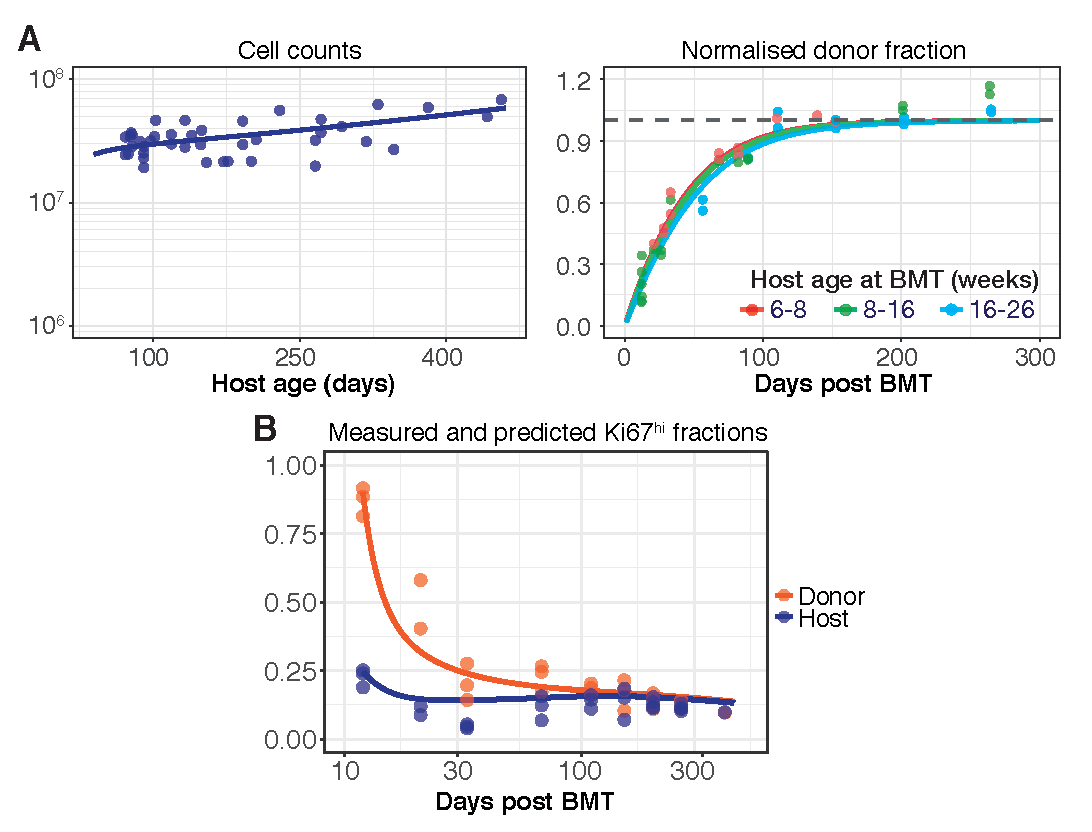
\includegraphics[scale = 0.9] {Results_FM.pdf}}
	\caption{\small \textbf{Dynamics of cell counts and donor fractions in FM B cell population using the best-fit `time-dependent' model.}  Model fits to the timecourse of cell counts (A) and donor fractions in FM B cells normalised to chimerism in T2 cells (B). Colours indicate different age-groups of recipient mice. The predictions for donor fractions for different age-gropus were generated using the  mode of the age within each group. (C) Host-age dependent changes in the net loss rate $\lambda(t)$ estimated from $\delta$ and $\rho$. (D) Predictions for the ki67$^+$ fractions within the host and donor compartment of FM B cells using the best-fit esimates from the time-dependent model in which $\delta$ declines with host age and $\rho$ is constant.}
	\label{fig:results_FM}
\end{figure}


\clearpage

%: Table 1
\begin{table}[h!]
	\begin{center}
		\renewcommand{\arraystretch}{1.25}
		\begin{tabular}{ l c c c c} 
			\toprule 
			& \multicolumn{3}{c}{\textbf{Model and $\Delta$AIC}} \\
			\cline{2-5}
			\textbf{Source}  &  {\small Time-dependent}  &  {\small Age-structured} & {\small Simple-homogeneous} & {\small Incumbent} \\ 
			\toprule
			Transitional 2 B cells      & 0      &  12.24 & 5.85 & 12.15$^\ast$  \\ 
			\hline
			\toprule 
		\end{tabular}
	\end{center}
	\caption{\small Comparison of AIC values for different models fitted to cell counts and donor fractions$^{\dagger}$ in FM B cells (Spleen + LN).}
	$^{\dagger}$ \footnotesize{Donor fractions in FM pool were normlised to the chimerism in T2 population. }\\
	$^\ast$ \footnotesize{Estimates for the number of incumbent cells are close to 0.}
	\label{tab:FM-AICs}
\end{table} 



%: Table 2
\begin{table}[h!]
	\begin{center}
		\renewcommand{\arraystretch}{1.25}
		\begin{tabular}{ l r l } 
			\toprule 
			\textbf{Parameter}  &  {\small Estimate}  &  {\small 95\% CI$^\dagger$} \\ 
			\toprule
			Total cell numbers at `t0' (in millions)      & 24.30      &  (10.88, 54.25)  \\ 
			Source influx at `t0'(in millions)           & 1.12      &  (0.95, 1.32)  \\
			Residence time at `t0' (days)      & 17.5      &  (7.5, 40.8)  \\ 
			Inter-division time (days)         & 56.1      &  (3.5, 899)  \\
			Half-life of $\delta(t)$ (days)    & 429       &  (127, 1449)  \\
			\hline
			\toprule 
		\end{tabular}
	\end{center}
	\caption{\small Parameter estimates from the best-fit `time-dependent' model for FM B cells (Spleen + LN).}
	$^\dagger$ \footnotesize Note: these are not bootsrap intervals but confidence intervals estimates by solving hessian matrix.
	\label{tab:FM-parestm}
\end{table} 


\clearpage

\section*{Methods}
\textbf{Mathematical models used to describe B cell population dynamics}
\paragraph*{Constant birth-death model:}
\textit{All cells behave identically at all times.} \\
In this model we assume that cells follow random birth-death processes to form a kinetically homogeneous population that self renews through homeostatic division and decays either by death or maturation. 
Per capita net loss rate `$\lambda$' is given by loss - proliferation ($\delta - \rho$)  and is assumed to be constant over time. \\
Abbereviated as CBDM

\be
\frac{dN}{dt} = \phi[t] \, - \lambda \, N(t)
\label{eq:SHM}
\ee

\paragraph*{Time-dependent model:} 
\textit{All cells behave identically at a given instant of time.} \\
This is also a homogeneous model where all cells obey the same rules of turnover. We assume that the fitness of the whole population changes over time/host-age, due to host-intrisic factors. 
The net loss rate $\lambda$ varies with time. We explored different forms of lambda changing with time and the best-fit was obtained with the very general form representing slow exponential decline in $\lambda$ with host age, $\lambda(t) = \lambda_0 \, e^{-r\,t}$.
Abbereviated as TDM

\be
\frac{dN}{dt} = \phi[t] \, - \lambda(t) \, N(t)
\label{eq:TDM}
\ee


\paragraph*{Age-structured model:} 
\textit{This is a heterogeneous model} \\
In this model the ability of individual cells to die or divide varies with their cell-age. 
The net loss rate $\lambda$ is a function of cell's age in the current lineage. 
Changes in fitness of individual cells with age could arise as a result of adaptive changes in cell-intrisic factors and/or conditioning that cells receive through micro-environmental inteactions (host intrisic factors) throughot their lifetime.
We explored different forms of $\lambda(a)$ changing with cell age and the best-fit was obtained by, $\lambda(a) = \lambda_0 \, e^{-r \,a} $.
The PDE described in eq.~\ref{eq:ASM} tracks the population dynamics of $N(a,t)$ over time.
We also assume that the fitness of individual cells is inherited by their daughter cells.
Abbereviated as ASM

\be
\frac{\partial{N(a,t)}}{\partial{a}} + \frac{\partial{N(a,t)}}{\partial{t}} = - \lambda(a) N(a,t),
\label{eq:ASM}
\ee

We solved Equation~\ref{eq:ASM} by the method of characteristics and using two boundary conditions. One is the constraint that the population density of cells of post-thymic age $a=0$, $N(t,0)$, at any time $t$  is simply the rate of source influx at that moment, $\phi(t)$. The second boundary condition is the population density with respect to cell age at time zero, $N(0,a) = g(a)$. We can then track both (i) the fate of the population present at time zero, $N_\text{init}(t,a)$,  and (ii) the fates of cells subsequently matured from T2 cells, $N_\phi(t,a)$;
\be
\begin{aligned} 
	N_\text{init}(t,a) &= g(a-t) \exp \bigg( - \int_0^t \lambda(\tau + a - t) \, d\tau \bigg), \, \text{for} \, a \ge t \\ 
	N_phi(t,a) &= phi(t-a) \exp \bigg (- \int_0^a \lambda(\tau) \, d\tau \bigg), \, \text{for}  \, a \le t \\ 
\end{aligned} 
\label{fig:PDEsolution}
\ee 
We consider three subsets: The host population generated pre-BMT $N_\text{init}^h (t,a)$, the host population post-BMT $N_phi^h (t,a)$, and the donor population post-BMT $N_phi^d (t,a)$. We add these subsets and integrate over cell age to obtain total cell counts.
\be
N_\text{total}(t) = \int_0^t \left ( N_\text{init}^h (t,a) + N_{\phi}^h (t,a)+ N_{\phi}^d (t, a) \right ) \, da 
\ee

We used the exponential ($\lambda(a) = \lambda_0 \, e^{-a/r}$) form for the net loss rate $\lambda$ decreasing with cell age. The population density of B cells with respect to cell age at time zero is unknown and we model it as $ g(a) = \, e^{p a} \, \phi_0 $. The free parameter $p$ can be positive or negative, such that older cells can initially be over- or under-represented compared to younger cells. This definition of $g(a)$ also ensures, for consistency, that $g(0)$ is the rate of influx at t0, $\phi_{0}$.  This quantity is unknown but can be expressed in terms of $g(a)$ and the initial pool size  $N_0$;
\be
\text{Total cell numbers} = \int_0^{t_0} g(a) \, da = \int_0^{t_0} e^{p a} \, \phi_0 \, da= N_{0} \implies   \phi_0 = \frac{N_{0} p}{e^{\,p \,t_a}-1} ,
\ee 
where the range of possible cell ages at host age $t_{0}$ is $0 \le a \le t_{0}$. 

Busulfan treatment results in  levels of chimerism that vary slightly across mice. To compare replacement across mice, we normalised the  fraction of cells in the periphery that were donor-derived to the chimerism in source compartment $\chi$.
\be
\text{Normalised donor fraction} \; f_{d} = \frac{N^d_{\phi}(t)} {\chi \, N_\text{total}(t)} \\
\ee 
To incorporate data from bone marrow transfers made in recipients with different ages, we tracked the changes in the numbers of (i) the cells present at $t_0$, until the host's age at BMT ($t_b$), which were present with age distribution $g(a)$ at time $t_{0}$; and (ii) the cells matured from T2 between $t_0$ and BMT. 
\be
\begin{aligned} 
	G(a) =\,\, & \left\{ 
	\begin{aligned} 
		&g(a-(t_b-t_0)) \,\, e^{\int_{0}^{t-t_0} \lambda(\tau) d\tau} \quad \quad \qquad a \geq t_b-t_0\ \\ 
		&\phi(t_b-t_0-a) \,\, e^{\int_{0}^{a} \lambda(\tau) d\tau} \quad \,\, \quad \quad \qquad a \le t_b-t_0\ 
	\end{aligned} 
	\right\} \\ 
\end{aligned} 
\\
\ee
The cell-age distribution at BMT  is therefore a composite function $G(a)$ that tracks the cells with age distribution $g(a)$ at the age of the mice with the earliest BMT, and also those cells exported from the thymus until the age of BMT. The model can therefore accommodate differences between mice in their age at BMT. Best-fit values of the unknown parameters - $N(0)$, $p$, $\lambda_0$, and $r$ were obtained by simultaneously fitting to the log-transformed cell counts and untransformed normalised donor fractions, in {\it R} using  the Nelder-Mead algorithm.


\paragraph{Incumbent model:}
\textit{This is also a heterogeneous model} \\
 The incumbent model (Hogan et al. 2015) considers that a B cell poulation is composed of kinetically distinct subpopulations - (i) an incumbent subset of older, self-renewing cells that are resistant to displacement by new cells and (ii) a displaceble subset that turns over with a constant rate `$\lambda$' and is replaced continuously by cohorts of new cells entering the pool.
 
\be
\begin{aligned}
 &\frac{dN_{\text{donor}}}{dt} = \chi \, \phi_0 \, e^{-\nu t} - \lambda \, N_{\text{donor}}(t) \\
 &\frac{dN_{\text{host}}}{dt} = (1-\chi) \, \phi_0 \, e^{-\nu t} - \lambda \, N_{\text{host}}(t)\\
 &\frac{dI}{dt}   = -\lambda_i I(t) 
\end{aligned}
\ee
 
As described in (Hogan et al. 2015), we solved these ODEs  to obtain total cell counts $N(t)$, with initial condition $N(0) - I(0) = N_{\text{donor}}(0) + N_{\text{host}}(0)$, where $N_{\text{donor}}(0)$, $N_{\text{host}}(0)$ and $I(0)$ are the numbers of donor, host and incumbent cells present at $t_0$, respectively. We accounted for different ages at BMT,  by tracking changes in initial donor population $N_{\text{donor}}(0)$ at different recipient ages. The initial cell counts and normalised donor fraction at the given age of BMT are then
\be
\begin{aligned}
&N(t_b) = \frac{\phi(t-t_0) \, \, (e^{(\lambda - \nu) (t_b-t_0)} - 1) + (\lambda-\nu) \, (N(0)-I(0)) + (\lambda-\nu) \, \, I(0) \, e^{(\lambda - \lambda_i) (t_b-t_0)}} {(\lambda-\nu) \,\, e^{\lambda (t_b-t_0)}} \\
\\
&f_d(t_b) = \frac{N(0) \,f_d(0) \, e^{-\nu (t_b-t_0)} }{N(t_b)}
\end{aligned}
\ee
and the total cell counts and normalised donor fraction as functions of host age are
\be
\begin{aligned}
&N(t) = \frac{\phi(t-t_0) \, \, e^{-\nu(t_b-t_0)} \, \,  (e^{(\lambda - \nu) (t-t_b)} - 1) + (\lambda-\nu) \, (N(t_b)-I(t_b)) + (\lambda-\nu) \, \, I(t_b) \, e^{(\lambda - \lambda_i) (t-t_b)}} {(\lambda-\nu) \,\, e^{\lambda (t-t_b)}}\\
\\
&f_d(t) = \frac{\phi(t-t_0) \, \, e^{-\nu(t_b-t_0)} \, \, (e^{(\lambda - \nu) (t-t_b)} - 1) + (\lambda-\nu) \,  N(t_b) \, f_d(t_b)}{ \phi(t-t_0) \, \, (e^{(\lambda - \nu) (t-t_b)} - 1) + (\lambda-\nu) \, (N(t_b)-I(t_b)) + (\lambda-\nu) \,\, I(t_b) \, e^{(\lambda -\lambda_i) \, (t-t_b)}}
\end{aligned}
\ee

The incumbent model has four free parameters ($N(0)$, $\phi_0$, $I(0)$ and $\lambda$) when fitted from t0 (the age of youngest animal at BMT) since fd(0) = 0.
 
 
\clearpage

\section*{Appendix}
\section*{Modelling chimerism dynamics in the source compartment}
In order to compare the inflitartion of donor cells into the FM pool across all animals that have varying levels of chimersim in their bone marrow cell populations, we normalise the fraction of donor cells in FM pool by dividing with the value of chimerism `$\chi$' in their immediate source i.e. T2 compartment.
Therefore the quantity, normalised donor fraction $f_{d}$, is independent of chimerism and is only sensitive to parameters that are common across animals.
We describe the changes in chimerism over time using a phenomenological function (equation~\ref{eq:chimerism})  that reasonably depicts the shape of the timecourse of fraction of donor cells across all animals.

\be
\chi(t) = \chi_{stable} \, (1 - e^{-q \,t}) 
\label{eq:chimerism}
\ee

Parameters `$\chi_{stable}$' and `q' are estimated by fitting the spline in equation~\ref{eq:chimerism} to the observed donor fractions in T2 compartment.


\section*{Modelling Source influx}
We assumed that the rate of influx from source $\psi$, stays constant and used the cell counts of Transitional 2 (T2) compartment as a proxy to estimate the number of cells maturing into the FM pool.  
Equation~\ref{eq:source}, is a spline that is used to describes the changes in T2 cells over time. 
Parameters $S_0$ and $\nu$ are estimated by fitting the spline in equation~\ref{eq:source} to the observed cell counts of T2 compartment.

\be
S(t) = S_0 \, e^{-\nu \, t}
\label{eq:source}
\ee
The counts of total, donor and host T2 cells entering the FM pool at any instant is given by equation~\ref{eq:influx}. The rate constant $\psi$ is estimated using model fits to cell counts and donor fractions.
\bea
\begin{aligned}
&\phi(t) = \psi \, S(t) \\
&\phi_{\text{donor}}(t) = \psi \, S(t) \, \chi(t)   \\
&\phi_{\text{host}}(t) = \phi(t) - \phi_{\text{donor}}(t) 
\end{aligned}
\label{eq:influx}
\eea

\begin{figure}[h!]
	\centerline{\includegraphics[scale = 0.9] {Source_FM.pdf}}
	\caption{\small \textbf{Dynamics of cell counts and chimerism in the source compartment (T2 cells).}  }
	\label{fig:Source_FM}
\end{figure}

\section*{Predicting the kinetics of ki67high fractions}

B cell subsets can be further divided in to recently divided (ki67$^+$) and quiscent (ki67$^-$) compartments. Dynamics of these compartments can  be tracked over time by studying changes in ki67 expression in the given subset.

\begin{figure}[htbp]
	\centerline{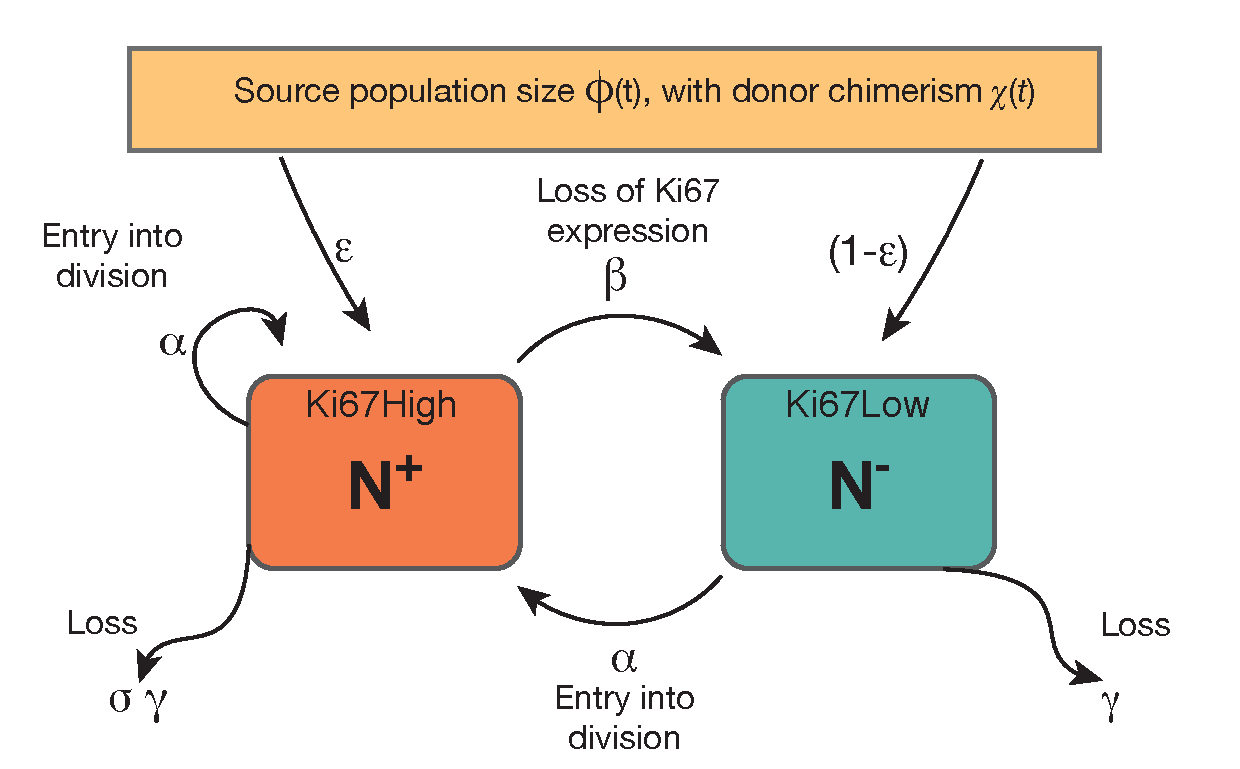
\includegraphics[scale = 0.5] {TwoComp_ki67.pdf}}
	\caption{Two compartment model for prolifeartion and loss of B cells using ki67 as a marker for dividing and recently divided cells \label{fig1}}
\end{figure}

This system is represented by the coupled ordinary differential equation described in eq.~\ref{general_ode}.

\begin{eqnarray}
\begin{aligned}
\frac{dY^+}{dt} &= \phi(t) \, \epsilon + \rho \, (2\, Y^- + Y^+) - \beta Y^+ - \sigma \delta^- Y^+ \\
\frac{dY^-}{dt} &= \phi(t) \, (1-\epsilon) - \rho Y^-  + \beta Y^+ - \delta^- Y^+
\end{aligned}
\label{general_ode}
\end{eqnarray}

Where, $\epsilon$ denotes the proportions of ki67$^+$ cells within the source influx.

$\kappa$ is the fraction ofki67$^+$ cells within the target population.
$\delta$ - the rate of loss (death + maturation). 
We depict the loss rates ki67$^-$ and ki67$^+$ cells as $\delta^-$ and $\delta^+$, respectively, since its possible that recently divided cells may have different susceptibility to die and/or mature as compared to quiescent cells. We assume a proportional relationship between these quantities, such that $\delta^+ = \sigma \, \delta^-$.

At $\sigma =1$, both ki67$^-$ and ki67$^+$ cells are lost with identical rates.

The resident times for individual cells within each compartment is given by, $\frac{1}{\delta}$.

$\rho$ - the rate of entry into division for both ki67$^-$ and ki67$^+$ cells.
Therefore, $\frac{1}{\rho}$ is the time taken for individual cells to divide.

$\beta$ - the rate of loss of ki67 expression.
$\frac{1}{\beta}$ - the average time taken for ki67Hi cells to become ki67Lo.
We estimate $\frac{1}{\beta}$ from the experimental data which is 3.5 days. 

We assumed that the influx from the source population changes very slowly relative to transition from ki67Hi to ki67Lo state, and therefore, both these compartments (Y$^+$ and Y$^-$) are in quasi-equilibrium. 
Estimates for  $\psi, \, \delta(t)$ and $\rho$ are obtained from the fits to cell counts and donor fractions. 
For the host and donor compartments $\phi_{\text{host}}(t)$ and $\phi_{\text{donor}}(t)$ were used respectively.
Initial cell counts of ki67$^-$ and ki67$^+$ were fixed from experimental obervations at t0 = 21 days post BMT. 
Kinetics of ki67$^+$ proportions were followed then after.
Mean values of experimental observations of $\epsilon$ and $\kappa$ were used to make these predictions.
$\beta$ and $\sigma$ were fixed at 1/3.5 and 1, respectively.



\clearpage



%: Table 1
\begin{table}[h!]
	\begin{center}
		\renewcommand{\arraystretch}{1.25}
		\begin{tabular}{ l | c c | c c | c c | c c } 
			\toprule 
			& \multicolumn{2}{c|}{\textbf{AIC}} & \multicolumn{2}{c|}{\textbf{Mean residence time}}  & \multicolumn{2}{c|}{\textbf{log(2)/r$^\ast$ estimates}}  & \multicolumn{2}{c}{\textbf{Inter-division time}} \\
			\cline{2-9}
			\textbf{Model}  &  {\small T1}  &  {\small T2} & {\small T1} & {\small T2} &  {\small T1}  &  {\small T2} & {\small T1} & {\small T2} \\ 
			\toprule
			Time-dependent            & 7.8   &  9.1 & 18(7, 44) & 17 (6, 54) & 250(46, 1300)  & 520(110, 2800) & 69(2, 2800) & 56 (3.5, 900)\\ 
			Age-structured            & 35   &  21 &  20(16, 26) & 33(21, 39) & NA  & NA &  89(36, 210) & 2000 (1300, 3300) \\ 
			\cline{4-9} 
			& \multicolumn{2}{c|}{\textbf{}} & \multicolumn{2}{c|}{\textbf{1/$\lambda_1^{\dagger}$ }}  & \multicolumn{2}{c|}{\textbf{$1/\lambda_2^{\dagger}$}} & \multicolumn{2}{c}{\textbf{}} \\
			\cline{4-9}
			constant birth-death       & 34  &  21 & 40(35, 47) & 34(30, 41) & -- & -- & -- & -- \\ 
			Incumbent                 & 34   &  21 & 39(34, 47) & 34(29, 40) & --  & -- & -- & -- \\ 
			Kinetic heterogeneity     & 34   &  21 & 41(37, 46) & 17 (6, 54) & 33(10,102) & 26(14, 47)  & -- & -- \\ 
			\hline
			\toprule 
		\end{tabular}
	\end{center}
	\caption{\small Comparison of AIC values for different models fitted to cell counts and donor fractions in FM B cells (Spleen + LN).}
	$^{\dagger}$ \footnotesize For the incumbent and constant birth-death model we only have $\lambda$ estimates. \\
	$^\ast$ \footnotesize r is the rate of change of residence-time with host-age or cell age, hence log(2)/r denotes the avearge time taken for men residence time to double. Changing $\rho$ with time or cell age gives (visually) poor fits hence not included in this analysis. \\
	\footnotesize NA - estimates for `r' are close to zero therefore log(2)/r $\sim$ NA/Inf. This shows that in this case there is very little or no effect of cell age on $\delta(a)$.
\label{tab:FMs}
\end{table} 

\blue{Note: Age-structured model gives visually bad fits for FM cells. \\
When  fitting FM cells with the incumbent model, size of the incumbent population is estimated to be $\approx$ 0, making it equivalent to constant birth-death model. When fitting MZ model the counts of incumbent cells are estimated $\approx 10^5$. }


%: Table 1
\begin{table}[h!]
	\begin{center}
		\renewcommand{\arraystretch}{1.25}
		\begin{tabular}{ l | c c | c c |c c |c c } 
			\toprule 
		& \multicolumn{2}{c|}{\textbf{AIC}} & \multicolumn{2}{c|}{\textbf{Mean residence time}}  & \multicolumn{2}{c|}{\textbf{log(2)/r$^\ast$ estimates}}  & \multicolumn{2}{c}{\textbf{Inter-division time}} \\
		\cline{2-9}
			\textbf{Model}  &  {\small T1}  &  {\small T2} & {\small T1} & {\small T2} &  {\small T1}  &  {\small T2} & {\small T1} & {\small T2} \\ 
			\toprule
			Time-dependent            & 32   &  66 & 19(7, 55)  & 32(11, 90) & 800(240, 2600) & 810(200,3200) & 28(7, 120) & 64(9,460) \\ 
			Age-structured            & 41   &  63 & 9(5, 16) & 11(5, 23)  & 1100(590, 2100) & 630(270, 1400) & 11(5, 22) & 15(6, 38) \\
			\cline{4-9} 
			& \multicolumn{2}{c|}{\textbf{}} & \multicolumn{2}{c|}{\textbf{1/$\lambda_1^{\dagger}$ }}  & \multicolumn{2}{c|}{\textbf{$1/\lambda_2^{\dagger}$}} & \multicolumn{2}{c}{\textbf{}} \\
			\cline{4-9}
			constant birth-death      & 44  &  68 & 111 (142, 100) & 90 (66, 125) & -- & -- & -- & -- \\ 
			Incumbent                 & 43   &  67 & 103(73, 171) & 67(45, 125) &  -- &  -- &  -- & --  \\ 
			Kinetic heterogeneity     & 40   &  66 & 270(106, 710) & 170(34, 840) & 73(52, 102) & 63(18, 210)& -- & -- \\ 
			\hline
			\toprule 
		\end{tabular}
	\end{center}
	\caption{\small Comparison of AIC values for different models fitted to cell counts and donor fractions in MZ B cells (Spleen).}
	$^{\dagger}$ \footnotesize For the incumbent and the constant birth-death model we only have $\lambda$ estimates. For the kinetic heterogenity model there are two subsets with different loss rates $\lambda_1$ and $\lambda_2$. \\
	$^\ast$ \footnotesize r is the rate of change of residence-time with host-age or cell age, hence log(2)/r denotes the avearge time taken for men residence time to double. Changing $\rho$ with time or cell age gives (visually) poor fits hence not included in this analysis. 
	\label{tab:MZs}
\end{table} 


\end{document}












